\nonstopmode
\documentclass[10pt,a4paper]{article}
\usepackage[utf8]{inputenc} % para poder usar tildes en archivos UTF-8
\usepackage[spanish]{babel} % para que comandos como \today den el resultado en castellano
\usepackage{a4wide} % márgenes un poco más anchos que lo usual
\usepackage{color}
\usepackage{gnuplottex}
%\usepackage{ccfonts,eulervm}
\usepackage{dot2texi}
\usepackage{tikz}
\usetikzlibrary{shapes,arrows}
\usepackage[T1]{fontenc}
\usepackage{listings}
\usepackage{xcolor}
\usepackage{amsmath}
\lstset { %
    language=C++,
    %backgroundcolor=\color{black!5}, % set backgroundcolor
                   basicstyle=\ttfamily,
                keywordstyle=\color{blue}\ttfamily,
                stringstyle=\color{red}\ttfamily,
                commentstyle=\color{green}\ttfamily,
                morecomment=[l][\color{magenta}]{\#}
}
\usepackage{float}
\usepackage{fancyhdr}
\pagestyle{fancy}
\thispagestyle{fancy}
\addtolength{\headheight}{1pt}
\lhead{AED3}
\rhead{TP2}
\usepackage[ruled,vlined,linesnumbered]{algorithm2e}
\usepackage[conEntregas]{caratula}
\renewcommand*{\algorithmcfname}{Algoritmo}

\begin{document}

\titulo{Trabajo Práctico II}
\subtitulo{Grupo 5}

\fecha{\today}

\materia{Algoritmos y Estructuras de Datos III}

\integrante{Aleman, Damian Eliel}{377/10}{damianealeman@gmail.com}
\integrante{Amil, Diego Alejandro}{68/09}{amildie@gmail.com}
\integrante{Barabas, Ariel}{775/11}{ariel.baras@gmail.com}
\integrante{Fern\'andez, Gonzalo Pablo}{836/10}{ralo4155@hotmail.com}

\maketitle


\tableofcontents

\newpage
\section{Introducción}
El presente informe apunta a documentar el desarrollo del Trabajo Práctico número 2 de la materia Algoritmos y Estructuras de Datos III, cursada correspondiente al segundo cuatrimestre del año 2013. Este trabajo pr\'actico consiste en la realización de un análisis teórico-experimental de un conjunto de problemas propuestos por la cátedra. Se requiere, para cada uno de los tres problemas, la implementación de un algoritmo que satisfaga criterios tanto de correctitud como de complejidad temporal.

Vamos a exponer, para cada uno de los problemas, los siguientes apartados:

\begin{itemize}
\item Una interpretación del enunciado, detallando ejemplos y/o casos particulares.
\item Una solución propuesta.
\item Un pseudocódigo que describa la implementación de dicha solución, junto con una explicación de su correctitud y una justificación de su complejidad.
\item Un apartado de testing, tanto de correctitud como de performance.
\end{itemize}


\newpage
\section{Pautas de Implementación}
El lenguaje elegido para la implementación de los algoritmos es \texttt{C++}. De ser necesario vamos a utilizar la biblioteca estandar del mismo y aclarar los costos de las operaciones en cuestión. En el caso de tener que implementar una clase propia para simplificar el código o proveer de cierto encapsulamiento, los costos de los métodos de la misma serán verificados y justificados. La estructura de directorios que utilizaremos para la implementación será la siguiente para todos los ejercicios:

\begin{verbatim}
\codigo
	 timer.h
	 tests.cpp
     \ejx
          ejx.cpp
          ejx.h
          Makefile
\end{verbatim}

El archivo \texttt{timer.h} contiene las funciones necesarias pera medir el
tiempo de ejecución de nuestros programas. Vamos a usar la función
\texttt{clock$\_$gettime} de la librería \texttt{time.h}. Estas funciones son
idénticas para las mediciones en todos los ejercicios. El archivo
\texttt{tests.cpp} contiene el código que testea los ejercicios. A este
programa se le pasan parámetros que utiliza para generar instancias de los
ejercicos y, con las funciones de \texttt{timer.h} mide el tiempo que tardan
en ejecutarse. Las funciones pedidas por la cátedra se encuentran en el
archivo \texttt{ejx.h}, y se incluyen en \texttt{ejx.cpp}. Este archivo
trabaja con entrada y salida standard de manera que, para ejecutar un programa
con su respectivo conjunto de casos, será suficiente con direccionarlo por
consola escribiendo \texttt{./ejx < ejx.in}. Obviaremos mencionar detalles
referentes a la carga de datos en las implementaciones. Cada archivo
\texttt{ejx.h} define los structs \texttt{entrada$\_$ejx} (inicializado a través
de la función \texttt{inicializar$\_$ejx} a partir de la entrada standard) y
\texttt{salida$\_$ejx} (devuelto por la función \texttt{resolver$\_$ejx}, la cual
toma una instancia del tipo \texttt{entrada$\_$ejx}). También se definen las
funciones \texttt{imprimir$\_$ejx}, la cual imprime una instancia de tipo
\texttt{salida$\_$ejx} por la salida standard y \texttt{generar$\_$instancia$\_$ejx}
la cual genera una instancia aleatoria de tipo \texttt{entrada$\_$ejx} a partir
de un parámetro como tamaño de la instancia. El código de \texttt{ejx.cpp}
lee entradas con \texttt{inicializar$\_$ejx} hasta recibir una entrada inválida.
Cada entrada la resuelve con \texttt{resolver$\_$ejx} y luego imprime el
resultado con \texttt{imprimir$\_$ejx}. El código de \texttt{tests.cpp} genera
instancias aleatorias con \texttt{generar$\_$instancia$\_$ejx}, las resuleve con
\texttt{resolver$\_$ejx} y luego imprime los tiempos de ejecución medidos.\\

Para modelar los ejercicios 2 y 3 decidimos implementar una clase grafo mediante listas de adyacencia y desarrollar los algoritmos necesarios como métodos de la misma. Contamos además con métodos auxiliares para simplificar el código, como por ejemplo \texttt{asociar(v,u,p)} que, dados dos nodos $v$ y $u$ crea una arista haciéndolos adyacentes con un peso $p$; o \texttt{vecinos(v)}, que devuelve un vector de todos los nodos que son vecinos a $v$.

Por ejemplo, el programa:

\begin{lstlisting}
	grafo g(3);
	g.asociar(1,2,7);
	g.asociar(2,3,4);
	g.asociar(3,1,2);
	grafo a = g.kruskal();
\end{lstlisting}

Nos va a crear un grafo \texttt{g} de tres nodos, va a crearle 3 aristas con pesos 7, 4 y 2, y luego va a generar un grafo \texttt{a} consistiendo en el AGM de \texttt{g}. 

\newpage
\section{Ejercicio 1}
\subsection{Interpretación del enunciado}
\par{Se tiene una imprenta en la que cada día deben realizarse determinados
trabajos. Los trabajos son realizados por las máquinas de la imprenta. Esta
imprenta cuenta con dos máquinas idénticas. Los trabajos son distintos, pero
pueden ser realizados por cualquiera de la dos máquinas siempre que se repete
un orden dado. Las máquinas deben prepararse para realizar determinados
trabajos y estas preparaciones tienen un costo, el cuál depende tanto del
trabajo a realizar como del estado de la máquina. Teniendo los trabajos
ordenados y los costos de preparación de las máquinas para cada trabajo, se
debe tomar cada trabajo, elegir la máquina en la que se realizará ese trabajo,
prepararla, y realizar el trabajo. El objetivo del ejercicio es desarrollar un
algoritmo que determine la mejor distribución de los trabajos entre las
máquinas que reduzca el costo total de la operación, es decir la suma de los
costos de cada preparación.}

\subsection{Resolucion}
\par{Sea $p(j)$ el problema de obtener la distribución óptima de $j$ trabajos
entre $2$ máquinas, definimos el problema derivado $p'(j,i)$ con $0<i<j$, el
cual consiste en obtener la distribución óptima de $j$ trabajos entre $2$
máquinas con la restricción de que los últimos trabajos realizados en cada
máquina sean $t_j$ y $t_i$. Notar que es indiferente en qué máquina se ejecuta
cada uno de estos. Definimos entonces la $distribucionOptima(j,i$)
como la distribución de costo mínimo con $j$ trabajos y el
trabajo $t_i$ como último trabajo de una de las máquinas. Notar que cualquier
distribución de $j$ trabajos siempre va a tener a $t_j$ como último trabajo en
una de las máquinas. Luego, la solución para el problema $p(j)$ es la solución
de costo mínimo de $p(j,i)$ para todo $i$, es decir:}

$$p(j) = \min_{\forall i} p(j,i) $$

El problema $p'$ se resolvió con programación dinámica mediante $distribucionOptima(j,i)$, que se calcula de la siguiente manera:
$$distribucionOptima(j,i) = \left\{
\begin{array}{c l}
 costo(0,1) & j = 1\\
 distribucionOptima(j-1,0) + costo(j-1,j) & i = 0 \land j > 1\\
 distribucionOptima(j-1,i) + costo(j-1,j) & 1 \le i < j-1 \land j > 1\\
 \displaystyle \min_{\forall k} distribucionOptima(j-1,k) + costo(k,j) & i = j-1 \land j > 1\\
\end{array}
\right$$

\par{Notar que siempre $i < j$. La entrada para ambos problemas es la cantidad
de trabajos y los costos de preparación de las máquinas para cada trabajo
definidos como:}
\begin{equation*}
$costo($i$,$j$) = Costo de preparar una máquina para realizar el trabajo $t_j$ luego
de haber realizado el trabajo $t_i$ (o no haber realizado ningún trabajo si
$i=0$). $0 \leq i < j
\end{equation*}\\
\par{A continuación se muestra el pseudocódigo de la solución para $p(j)$,
resolviendo $p'(j,i)$.}\\
\begin{algorithm}[H]
	\caption{Algoritmo de Ejercicio 1}
	\KwData{\textbf{int} $cantTrabajos$, $costos$}
	$distribucionOptima(1,0) \longleftarrow costo(0,1)$\\
	\For{$j \in \{2..cantTrabajos\}$}{
		
		$distribucionOptima(j,0) \longleftarrow distribucionOptima(j-1,0) + costo(j-1,j)$\\
		$distribucionOptima(j,j-1) \longleftarrow distribucionOptima(j-1,0) + costo(0,j)$
		
		\For{$i \in \{1..j-2\}$}{
	
			$distribucionOptima(j,i) \longleftarrow distribucionOptima(j-1,i) + costo(j-1,j)$\\
			$distribucionOptima(j,j-1) \longleftarrow min(distribucionOptima(j,j-1), distribucionOptima(j-1,i) + costo(i,j))$\\
		}
	}
	\textbf{return} $ \displaystyle \min_{\substack{\forall i}} distribucionOptima(cantTrabajos,i) $\\
\end{algorithm}

\subsection{Demostración de Correctitud}

\textbf{Propiedad 1 -}  \emph{ Existe un $i$ tal que la solución del problema $p'(j,i)$
es solución de $p(j)$. }\\

\textbf{Demostración:} Es inmediato ver que alguna solución del problema $p(j)$ pertenece al
conjunto de las soluciones de $p(j,i)$ para algún $i$. Dado que $p(j)$ no tiene
la restricción del trabajo realizado como último en la otra máquina, la solución al
problema $p(j)$ es la solución de $p(j,i)$ con menor costo:
$$p(j) = \min_{\forall i} p(j,i)$$

\textbf{Propiedad 2 -} \emph{$ (\forall i < j) \quad distribucionOptima(j,i) $ devuelve una de las distribuciones con menor costo dados
j trabajos e i como último trabajo.}\\

\textbf{Demostración:}
Vamos a demostrar por inducción en j.


\textbf{Caso base. Si $j = 1:$}
Queremos ver que $ (\forall i < j) \quad distribucionOptima(1,i) $ devuelve una de las distribuciones con menor costo dados
$1$ trabajo e i como ultimo trabajo. Notar que siempre $i < j$ , por lo tanto $i$ debe ser $0$. 
Hay sólo una forma de configurar un trabajo en las dos máquinas, que este trabajo sea el único de una máquina
y la otra máquina este libre de trabajos, es decir que el costo de la distribución optima es igual a el costo de preparar
el trabajo $1$ luego del trabajo $0$ que es los mismo que \\
$distribucionOptima(1,0) = costo(0,1)$.
Luego, queda demostrado el caso base.\\


\textbf{Paso Inductivo:} Se dividirá la demostración en dos casos :\\

\textbf{Caso $i <  j-1$:} 

Definimos a $ distribucionOptima(j,i) $ = 
$distribucionOptima($j$-1,$i$) + costo($j$-1,$j$) & $\\
Supongamos que no es la distribución optima y lleguemos a un absurdo. Decir que es la distribución es óptima es lo mismo que afirmar que
que no hay ninguna distribución de $j$ trabajos con $i$ como último trabajo que cueste menos que $ distribucionOptima(j,i) $.
Sea $d_2$ la distribución que cuesta menos que $ distribucionOptima(j,i) $ y tiene j trabajos e i como último trabajo.
Luego por como se 
define la preparación de los trabajos,en $d_2$ el trabajo $j$ está al final de una máquina (y como $(i < j-1) \Rightarrow i \neq j $ )
y el trabajo $i$ está en la otra máquina. De esta manera, si quitamos el trabajo $j$, obtenemos una configuración de $j-1$ trabajos con $i$
como último trabajo, llamemosla $d_{2'}$.

\begin{align*}
\text{Por lo tanto}
\qquad costo (d_2) &= costo (d_{2'}) + costo(j-1,j) \\
\text{y como }
 \qquad costo(d_2) &<  distribucionOptima(j,i) \\ 
\text{entonces}
 \qquad costo (d_{2'}) &< distribucionOptima(j-1,i). Absurdo. 
\end{align*}

\textbf{Caso $i = j-1:$}

Definimos a $ distribucionOptima(j,i) $ =  
\displaystyle \min_{\substack{\forall i \in \{0..j-1\}}} \ $distribucionOptima($j$-1,$i$) + costo($i$,$j$)$
 & \\
 
Supongamos que no es la distribución optima y lleguemos a un absurdo.
Sea $d_2$ la distribución que cuesta menos que $ distribucionOptima(j,i) $ y tiene $j$ trabajos e $i$ como último trabajo.
Luego por como se 
define la preparación de los trabajos,en $d_2$ el trabajo $j$ está al final de una máquina (y como $(i = j-1) \Rightarrow i \neq j $ )
y el trabajo $i$ está en la otra máquina.
De esta manera, si quitamos el trabajo j, obtenemos una configuración de $j-1$ trabajos con $j-1$
y algún k (con $ 0 \le k < j-1$) como últimos trabajos en las dos máquinas, llamemosla $d_{2'}$.

\begin{align*}
\text{Por lo tanto}
\qquad costo (d_2) &= costo (d_{2'}) + costo(k,j)  \text{para algun k (con }  0 \le k < j-1) \\
\text{y como }
 \qquad costo(d_2) &<  distribucionOptima(j,i) \\ 
\text{entonces}
 \qquad costo (d_{2'}) &< distribucionOptima(j-1,k). 
\end{align*}

Absurdo pues por la definición
\displaystyle \min_{\substack{\forall k \in \{0..j-1\}}} \ $distribucionOptima($j$-1,$k$) + costo($k$,$j$)$. \\

\textbf{Corolario de Propiedad 2 -} \emph{$ distribucionOptima(cantTrabajos,i) $ devuelve una de las distribuciones con menor costo dados
cantTrabajos trabajos e i como ultimo trabajo.)}\\

Ahora veremos que el algoritmo retorna la distribución óptima según como la definimos.\\
\textbf{Caso $j = 1:$} En la línea $1$ del pseudocódigo se asigna la distribución óptima según como la definimos:
$$costo(1,0)$$
\textbf{Para $j > 1$:}
\textbf{Caso $i = 0$:} En la línea $3$ del pseudocódigo se asigna la distribución óptima según como la definimos:
$$distribucionOptima(j-1,0) + costo(j-1,j)$$
\textbf{Caso $1 \le i < j-1:$} En la línea $6$ del pseudocódigo se asigna la distribución óptima según como la definimos:
$$distribucionOptima(j-1,i) + costo(j-1,j)$$
\textbf{Caso $i = j-1:$} Sea $g(i) = distribucionOptima(j-1,i) + costo(i,j).$
En este caso se inicializa $distribucionOptima(j,j-1)$ en la linea $4$ con $g(0)$.
Luego en el ciclo interno se compara el valor actual de $distribucionOptima(j,j-1)$ con los valores
$g(i)$ para todo $ 1 \le i \le j-2 $. 


\subsection{Cota de Complejidad}
Para demostrar la complejidad del algoritmo, vemos que la incialización de la matriz de costos
tiene una complejidad de $O(n^2)$, con $n$ la cantidad de trabajos, ya que completa una matriz de $n^2$ elementos con dos ciclos anidados.

Luego, el algoritmo completa la matriz de $distribucionOptima$, con dos ciclos anidados. En cada uno de estos ciclos,
las variables de iteración se van incrementando de a uno y cada una debe iterar
en un numero menor o igual a la cantidad de trabajos.
\textbf{Cada asignación tiene una complejidad de $O(1)$, ya que al momento de la asignación (en la iteración $j$)
$distribucionOptima(j-1,i)$ ya está calculada y guardada en la matriz.}\\

\begin{algorithm}[H]
	\caption{Algoritmo de Ejercicio 1}
	\KwData{\textbf{int} $cantTrabajos$, $costos$}
	$distribucionOptima(1,0) \longleftarrow costo(0)(1)$	         \tcc*[r]{$O(1)$}
	\For{$j \in \{2..cantTrabajos\}$ \tcc*[r]{$O(n)$}}{	
		
		$distribucionOptima(j,0) \longleftarrow distribucionOptima(j-1)(0) + costo(j-1)(j)$\\ 	
		$distribucionOptima(j,j-1) \longleftarrow distribucionOptima(j-1)(0) + costo(0)(j)$		
		
		\For{$i \in \{1..j-2\}$ \tcc*[r]{$O(n)$} }{	
	
			$distribucionOptima(j,i) \longleftarrow distribucionOptima(j-1,i) + costo(j-1,j)$\\	${O(1)}$
			$distribucionOptima(j,j-1) \longleftarrow min(distribucionOptima(j,j-1), distribucionOptima(j-1)(i) + costo(i)(j))$\\
		}
	}
	\textbf{return} $ \displaystyle \min_{\substack{\forall i}} distribucionOptima(cantTrabajos,i) $	\tcc*[r]{$O(n)$}
\end{algorithm}

Luego la complejidad del algoritmos es $ O(n^2) + n * O(n) + O(n) = O(n^2).$

\subsection{Implementación}

\begin{lstlisting}
salida_ej1 resolver_ej1(entrada_ej1 entrada) {
  int cantTrabajos = entrada.n;
  vector<vector<int> > costo = entrada.matriz;

  //En la posicion i j está el costo de la configuración optima para
  //los primeros i trabajos con el trabajo j como ultimo de la otra máquina.
  vector < vector<par> > 
	distribucionOptima(cantTrabajos+1,vector<par> (cantTrabajos) );
  distribucionOptima[1][0] = make_pair(costo[0][1],0);
  
  for ( int j = 2; j <= cantTrabajos; ++j ) {
    distribucionOptima[j][0] = make_pair (distribucionOptima[j-1][0].first 
					+ costo[j-1][j],j-1);
    distribucionOptima[j][j-1] = make_pair (distribucionOptima[j-1][0].first
					+ costo[0][j],0);
    for ( int i = 1; i < j-1 ; ++i ) {
      distribucionOptima[j][i] = make_pair(distribucionOptima[j-1][i].first
						    + costo[j-1][j],j-1);
      int costoAlternativo = distribucionOptima[j-1][i].first + costo[i][j];
      if (costoAlternativo < distribucionOptima[j][j-1].first) {
	    distribucionOptima[j][j-1] = make_pair(costoAlternativo,i);
      }
    }
  }

  vector<int> tEnMaq1(0);
  int k = 0;
  int C = distribucionOptima[cantTrabajos][0].first;

  int elAnterior = cantTrabajos-1;
  int ultimoOtraMaquina = 0;
  for (int i=1; i<cantTrabajos; i++) {
      if (distribucionOptima[cantTrabajos][i].first < C) {
	C = distribucionOptima[cantTrabajos][i].first;
	elAnterior = distribucionOptima[cantTrabajos][i].second;
	ultimoOtraMaquina = i;
      }
  }
  
  //cout << "el anterior es " << elAnterior << endl;

  int trabajoEnMaquina = cantTrabajos;	
  tEnMaq1.push_back(trabajoEnMaquina);
  k++;

  while (elAnterior != 0){
    tEnMaq1.push_back(elAnterior);
    k++;
    trabajoEnMaquina = elAnterior;
    while (ultimoOtraMaquina > elAnterior) {
      ultimoOtraMaquina = 
	      distribucionOptima[ultimoOtraMaquina][elAnterior].second;
      }
    elAnterior = 
	distribucionOptima[trabajoEnMaquina][ultimoOtraMaquina].second;
}

  vector<int> e = vector<int>(k);
  for (int i=0; i<k; i++) {
	  e[i] = tEnMaq1[k-i-1];
  }

  //cout << "vector de trabajos" << endl;
  //mostrarVec(e);
  
  //cout << "matriz de cofiguracion Optima" << endl;
  //mostrarMatriz(distribucionOptima,cantTrabajos+1,cantTrabajos);
  //cout << endl;

  salida_ej1 salida(C, k, e);
  return salida;
}
\end{lstlisting}
\newpage
\subsection{Testing de Correctitud}

Los tests expuestos a continuación fueron diseñados con el fin de verificar
diferentes casos particulares que pudimos identificar. Para cada test vamos
a exponer la entrada, la salida y, en caso de que sea necesario, una
justificaci\'on de la correctitud de la soluci\'on.\\

\noindent\textbf{Test$\#$1}\\
\textbf{Caracterización:} Un solo trabajo.\\
\textbf{Input:}\\ \texttt{1\\5}\\
\textbf{Output:} \texttt{5 1 1}\\
\textbf{Status:} OK. Asigna el único trabajo a la máquina 1 y el costo total
es el costo de ubicar el trabajo 1 en la máquina 1.\\

\noindent\textbf{Test$\#$2}\\
\textbf{Caracterización:} Dos trabajos que conviene ubicar uno trás otro.\\
\textbf{Input:}\\ \texttt{2\\3\\8 3}\\
\textbf{Output:} \texttt{6 2 1 2}\\
\textbf{Status:} OK. Ubica ambos trabajos en la misma máquina y el costo
total es el costo de ubicar el trabajo 1 en una máquina vacía más el costo
de ubicar el trabajo 2 tras el trabajo 1.\\

\noindent\textbf{Test$\#$3}\\
\textbf{Caracterización:} Dos trabajos que conviene ubicar como primeros en
una máquina.\\
\textbf{Input:}\\ \texttt{2\\3\\3 8}\\
\textbf{Output:} \texttt{6 1 2}\\
\textbf{Status:} OK. Ubica un trabajo en cada máquina y el costo total es la
suma de los costos de ubicar cada trabajo como primer trabajo de una máquina.\\

\noindent\textbf{Test$\#$4}\\
\textbf{Caracterización:} Todos los costos son iguales.\\
\textbf{Input:}\\ \texttt{5\\1\\1 1\\1 1 1\\1 1 1 1\\1 1 1 1 1}\\
\textbf{Output:} \texttt{5 5 1 2 3 4 5}\\
\textbf{Status:} OK. Cualquier distribución de trabajos en máquinas tiene
costo igual a 5.\\

\noindent\textbf{Test$\#$5}\\
\textbf{Caracterización:} Todos los costos son distintos (incrementando).\\
\textbf{Input:}\\ \texttt{3\\1\\2 3\\4 5 6}\\
\textbf{Output:} \texttt{8 1 3}\\
\textbf{Status:} OK.\\

\noindent\textbf{Test$\#$6}\\
\textbf{Caracterización:} Todos los costos son distintos (decrementando).\\
\textbf{Input:}\\ \texttt{3\\6\\5 4\\3 2 1}\\
\textbf{Output:} \texttt{11 3 1 2 3}\\
\textbf{Status:} OK.\\

\noindent\textbf{Test$\#$7}\\
\textbf{Caracterización:} Varios trabajos que conviene ubicar uno tras otro.\\
\textbf{Input:}\\ \texttt{5\\1\\8 1\\8 8 1\\8 8 8 1\\8 8 8 8 1}\\
\textbf{Output:} \texttt{5 5 1 2 3 4 5}\\
\textbf{Status:} OK. Ubica todos los trabajos en la misma máquina.\\

\noindent\textbf{Test$\#$8}\\
\textbf{Caracterización:} Varios trabajos que conviene ubicar intercalados.\\
\textbf{Input:}\\ \texttt{5\\1\\1 8\\8 1 8\\8 8 1 8\\8 8 8 1 8}\\
\textbf{Output:} \texttt{5 3 1 3 5}\\
\textbf{Status:} OK. Ubica los trabajos impares en la misma máquina (por lo
tanto, ubica los pares en la otra).\\

\noindent\textbf{Test$\#$9}\\
\textbf{Caracterización:} La subsolución de la solución óptima no es solución
óptima para su subproblema asociado.\\
\textbf{Input:}\\ \texttt{3\\5\\3 5\\1 8 8}\\
\textbf{Output:} \texttt{11 1 3}\\
\textbf{Status:} OK. La solución óptima consiste en ubicar los trabajos 1 y 2 en
una máquina y el trabajo 3 en otra. Sin embargo, la subsolución de dos trabajos
que ubica a los trabajos 1 y 2 en la misma máquina no es solución óptima del
subproblema asociado (distribuír los trabajos 1 y 2 entre las 2 máquinas de
forma óptima.)\\

\newpage
\subsection{Testing de Performance}

\par{Realizamos un gráfico comparando la sucesión de tiempos obtenida con una función cuadrática, pues demostramos que la complejidad del algoritmo es cuadrática.
La función $f = n^2$, donde $C = \frac{1}{20500000}$. Se midió el tiempo con n desde 1 hasta 1000 con saltos de a 10 (con 100 mediciones por cada n).}


\begin{figure}[H]
\centering
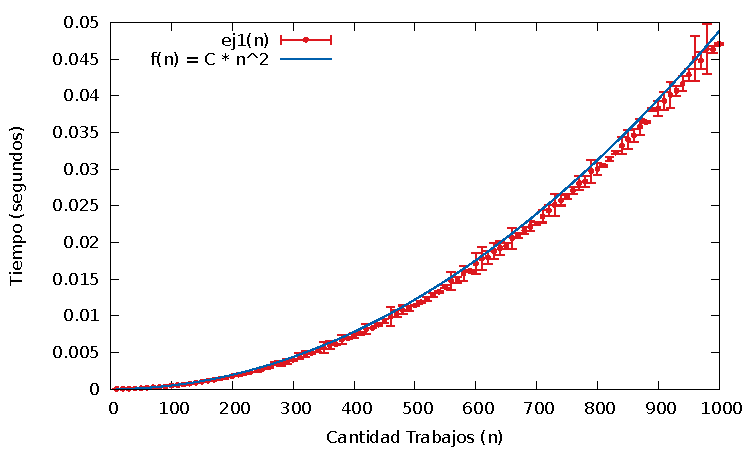
\includegraphics{imgs/ej1_1000_10_100.pdf}
\caption{Test Performance: Tiempo(s) vs Cantidad de Trabajos.}
\end{figure}

\par{Hay que notar que las franjas para cada tamaño de entrada muestran el desvío estandar de todos los valores conseguidos para ese tamaño, esto nos pareci\'o mucho m\'as significativo que simplemente mostrar el máximo y el m\'inimo, ya que estos valores pueden variar mucho por otros procesos que pueda estar ejecutando la computadora a la vez.}


\newpage
\section{Ejercicio 2 - A}

\subsection{Interpretación del enunciado}

El siguiente problema trata sobre el almacenamiento y la transmisión de datos entre servidores. Se tiene un conjunto de $n$ servidores interconectados de a pares a través de $m$ enlaces. Un servidor $v_i$ puede transmitirle información a otro servidor $v_j$ de manera directa si y sólo si existe un enlace entre dichos servidores. Si no, la información deberá llegar a $v_j$ pasando por otros servidores intermedios.

El tiempo que tarda la información en transmitirse a través de un enlace es constante para todos los enlaces, aunque el uso de estos enlaces tiene un costo que depende de cada enlace en cuestión. Se cumple que para todo par de servidores en la red, el costo de enviar información en un sentido es el mismo que el de enviarla en el sentido contrario.

En esta red de servidores, se llama ``broadcast'' al proceso de replicar información entre todos los servidores, de manera que después de un determinado tiempo, todos los servidores de la red tengan la misma información. Para hacer esto, se designa a un servidor como $master$, que es el único que inicialmente tiene la información a replicar. Este servidor $master$ va a copiar la información a todos aquellos servidores que están conectados directamente a él.

Cada vez que un servidor recibe una actualización, envía la información recibida a todos los otros servidores conectados a él (exceptuando al servidor del cual recibió la actualización). Todas las transmiciones realizadas por un servidor se hacen simultáneamente. Esto se repite hasta que todos los servidores de la red tengan la misma información.

El objetivo de este ejercicio es el de desarrollar un algoritmo que determine un conjunto de enlaces en el que el costo de mantenerlos todos sea el mínimo y a su vez, la actualización pueda llegar desde el servidor $master$ a cada uno de los demás servidores.

\subsection{Resolución}

Se modelará la situación a través de un grafo ponderado no dirigido en el que cada nodo representará un servidor y cada arista entre un par $v1$, $v2$ de nodos representará un enlace entre los servidores correspondientes a $v1$ y $v2$. Se le asignará a cada arista el peso equivalente al costo de mantener su correspondiente enlace. Se asume que el grafo es conexo, ya que se parte de que todos los servidores están interconectados. 

Por ejemplo, el siguiente grafo:\\

\begin{center}
\begin{dot2tex}
graph graphname{
	rank=same;
	rankdir="LR";
	splines=line;
	{rank=same; 1 5}
	{rank=same; 2 6}
	{rank=same; 3 7}
	{rank=same; 4 8}
	1 -- 2 [label=5];
	2 -- 3 [label=17];
	3 -- 4 [label=3];
	1 -- 5 [label=24];
	5 -- 6 [label=8];
	6 -- 7 [label=16];
	7 -- 8 [label=19];
	4 -- 8 [label=7];
	2 -- 6 [label=51];
	3 -- 7 [label=21];
	5 -- 2 [label=29];
	2 -- 7 [label=3];
	7 -- 4 [label=65];
}
\end{dot2tex}
\end{center}

%revisar por que los nodos están a diferentes alturas
representa a una red con 8 servidores donde, por ejemplo, el costo de hacer una transmición entre los nodos 2 y 6 es de 51. 
%Si se asigna al
%~ servidor número 7 para ser el servidor $master$, los datos se
%~ transmitirían de la siguiente manera:
%~ 
%~ 
%~ \begin{center}
%~ \begin{dot2tex}
%~ graph graphname{
	%~ rankdir="LR";
	%~ ratio="compress";
	%~ nodesep=0.0005;
	%~ size="0.50,0.50";
	%~ 7 -- 2;
	%~ 7 -- 3;
	%~ 7 -- 4;
	%~ 7 -- 6;
	%~ 7 -- 8;
	%~ 2 -- 1;
	%~ 2 -- 5;
%~ }
%~ \end{dot2tex}
%~ \end{center}
%~ 
%~ Dado que se pide que los subproblemas de encontrar el conjunto de enlaces
%~ de costo mínimo y de seleccionar el servidor $master$ para minimizar el tiempo
%~ de ``broadcast'' se resuelvan por separado, se implementarán 2 algoritmos
%~ independientes para resolverlos.}

Para resolver este problema se debe, dado un conjunto de $n$ servidores y $m$ enlaces, encontrar un subconjunto de $m' < m$ enlaces tales que sea posible conectar todos los $n$ servidores entre si, pero utilizando los enlaces de menor costo posible. Esto se puede pensar como, dado un grafo conexo con pesos en sus aristas, encontrar un árbol generador mínimo del mismo. Vale aclarar que dado un grafo $G$, puede haber más de un AGM del mismo. En este ejercicio no hay requerimientos específicos sobre cuál AGM devolver. Para el grafo de la figura anterior, un AGM posible podría ser el siguiente:
 
%~ desde: 2 - hasta: 7 - peso: 3
%~ desde: 3 - hasta: 4 - peso: 3
%~ desde: 1 - hasta: 2 - peso: 5
%~ desde: 4 - hasta: 8 - peso: 7
%~ desde: 5 - hasta: 6 - peso: 8
%~ desde: 6 - hasta: 7 - peso: 16
%~ desde: 2 - hasta: 3 - peso: 17

\begin{center}
\begin{dot2tex}
graph graphname{
	rank=same;
	rankdir="LR";
	splines=line;
	{rank=same; 1 5}
	{rank=same; 2 6}
	{rank=same; 3 7}
	{rank=same; 4 8}
	1 -- 2 [label=5];
	2 -- 3 [label=17];
	3 -- 4 [label=3];
	1 -- 5 [label=24, style=dotted];
	5 -- 6 [label=8];
	6 -- 7 [label=16];
	7 -- 8 [label=19, style=dotted];
	4 -- 8 [label=7];
	2 -- 6 [label=51, style=dotted];
	3 -- 7 [label=21, style=dotted];
	5 -- 2 [label=29, style=dotted];
	2 -- 7 [label=3];
	7 -- 4 [label=65, style=dotted];
}
\end{dot2tex}
\end{center}

Optamos por implementar el Algoritmo de Kruskal para obtener el AGM. Ya que el mismo cumple con la cota de complejidad temporal requerida en este problema. Este algoritmo
itera sobre las aristas agregando al resultado la arista de menor peso que no
forme ciclos. Para esto, se ordenan las aristas según su peso (para así
obtener en tiempo constante la arista de menor peso) y luego se las agrega
hasta formar un árbol. A continuación se muestra el pseudocódigo del algortimo
de Kruskal:\\

\begin{algorithm}[H]
	\caption{Algoritmo de Kruskal}
	\KwData{\textbf{Grafo} $G$}
	$G.aristas \longleftarrow$ ordenar$\_$por$\_$peso$\_$asc($G.aristas$)\\
	\textbf{vector<arista>} $res \longleftarrow \emptyset$\\
	\ForEach{$e \in G.aristas$}{
		\If{!forma$\_$ciclo($e$, $res$)}{
		$res \longleftarrow res \cup e$\\
		}
	}
	\textbf{return} $res$\\
\end{algorithm}

\subsection{Demostración de Correctitud}

\textbf{Propiedad 1 -} \emph{Un árbol generador mínimo del grafo que representa
la red es una solución al problema.}\\

\par{Un AGM es un árbol y por lo tanto existe un único camino entre todo par
de vértices; entonces se cumple que cualquier servidor puede enviar
información y que todo otro servidor recibirá dicha información eventualmente.
El costo de mantener todos los enlaces es la suma de los costos de mantener
cada enlace, es decir es equivalente al peso del árbol generador; y, como de
todos los posibles árboles generadores, se toma el de mínimo peso, podemos
asegurar que estamos tomando el conjunto de enlaces de menor costo.}\\

\textbf{Propiedad 2 -} \emph{El algoritmo de Kruskal genera una árbol generador
mínimo a partir de un grafo conexo con pesos en los ejes.}\\

\par{Está demostrado que el algoritmo de kruskal es correcto (citar
demostración) y devuelve un AGM. La demostración de correctitud consiste en
probar que el resultado es un árbol ya que la cantidad de aristas es una menos
que la cantidad de nodos y no forman ciclos ya que sólo se agregan las aristas
que no forman ciclos con el conjunto de aristas ya agregado. La demostración
de optimalidad se basa en suponer que existe un árbol generador de menor
peso que el que devuelve el algoritmo de Kruskal y se llega a un absurdo,
ya que Kruskal elige siempre las aristas de menor peso.}

\subsection{Cota de Complejidad}

\par{La complejidad del algortimo es la complejidad de Kruskal.}

\subsection{Implementación}

Nuestra implementación del algoritmo de Kruskal es la siguiente:
\begin{lstlisting}
  
  grafo kruskal(){
    disjointSet ds(this->cantNodos);
    vector<arista> res;
    /*Ordeno la lista de aristas para Kruskal */
    sort(this->aristas.begin(), this->aristas.end()); 
        
    int i = 0;  /* Indice de arista que itero */
    int j = 0;  /* Cantidad de aristas que agrege */
    
    while ( j < this->cantNodos-1 ) {
      if(!ds.sameSet(this->aristas[i].nodo1, this->aristas[i].nodo2)){
        ds.union_by_rank(this->aristas[i].nodo1, this->aristas[i].nodo2);
        res.push_back(this->aristas[i]);
        j++;
      }
      i++;
    }
    
    /* Armo el grafo para devolver */
    grafo g_res(this->cantNodos);
    for(int i = 0; i < res.size(); ++i)
      g_res.asociar(res[i].nodo1+1, res[i].nodo2+1, res[i].peso);
    
    return g_res;
  }
\end{lstlisting}

Notar que fue necesario agregar a nuestro programa una parte que creara un grafo para poder devolver algo que la segunda parte del ejercicio 2 pudiera procesar sin tener que volver a leer la entrada.


\newpage
\section{Ejercicio 2 - B}
\subsection{Interpretación del enunciado}
Para este ejercicio se pide, dada una red de servidores, los cuales están todos interconectados entre sí con un conjunto de enlaces de costo mínimo; encontrar un servidor tal que, al designarlo $master$ de la red, se garantice que el broadcast se complete en el menor tiempo posible. Vale destacar que este problema toma como entrada la salida del anterior.

Veamos algunos ejemplos. Si consideramos la solución propuesta anteriormente, tenemos que la misma es el siguiente árbol:

\begin{center}
\begin{dot2tex}
graph graphname{
	rank=same;
	rankdir="LR";
	splines=line;
	{rank=same; 1 5}
	{rank=same; 2 6}
	{rank=same; 3 7}
	{rank=same; 4 8}
	1 -- 2 [label=5];
	2 -- 3 [label=17];
	3 -- 4 [label=3];
	4 -- 8 [label=7];
	5 -- 6 [label=8];
	6 -- 7 [label=16];
	2 -- 7 [label=3];
}
\end{dot2tex}
\end{center} 

Veamos entonces, cuanto tardaría en completarse un broadcast para cada servidor. El enunciado dice que el tiempo de transimisón de cada enlace es el mismo dados dos servidores cualesquiera que estén conectados. Por lo que podemos asumir que, si tenemos un árbol $A$ y un vertice $v$, el tiempo total del broadcast es la altura del árbol $A$ tomando a $v$ como raiz del mismo. Para el árbol del ejemplo, los tiempos totales de broadcast correspondientes para cada servidor son los siguientes:

\begin{center}
  \begin{tabular}{ c | c | c | c | c | c | c | c | c}
    servidor & 1 & 2 & 3 & 4 & 5 & 6 & 7 & 8 \\ \hline
    tiempo   & 4 & 3 & 4 & 5 & 6 & 5 & 4 & 6 \\
    \end{tabular}
\end{center}

Se observa que en este caso la única solución óptima es seleccionar como $master$ al servidor número 2. Podemos ver que obtuvimos los peores resultados cuando seleccionamos como $master$ a los servidores 5 y 8 que coincidentemente son hojas del árbol. 

\subsection{Resolución}

La pregunta que nos surge entonces es: Dado un árbol, ¿cuál nodo deberíamos seleccionar como raíz del mismo para garantizar que este árbol tenga altura mínima? Propondremos y demostraremos que el nodo óptimo es aquel que se encuentra a la mitad del camino más largo del árbol. Nuestra solución va a implementar un algoritmo para encontrarlo en
tiempo lineal. 

Nuestra resolución implementa el siguiente procedimiento. Primero se realiza un BFS partiendo desde el nodo raíz del árbol. Nos vamos a quedar con el nodo más lejano que podamos encontrar a la raíz. De ser más de uno, nos vamos a quedar con el último que hayamos recorrido. Llamaremos a este nodo $v_1$.

Luego, vamos a hacer otro BFS partiendo desde el nodo $v_1$, y nos vamos a quedar con el nodo más alejado a $v_1$ que encontremos, al cual llamaremos $v_2$. Luego, el camino más largo del árbol es el que está comprendido entre los nodos $v_1$ y $v_2$. Haciendo un DFS\footnote{Un DFS con algunas modificaciones para encontrar el camino y luego devolver el nodo medio de este.} desde $v_1$ hasta $v_2$ vamos a ir recorriendo este camino. El nodo que buscamos es aquel que se encuentra en la mitad de este camino.

\newpage
Un pseudocódigo de lo anteriormente descripto es el siguiente:\\

\begin{algorithm}[H]
	\caption{Busqueda del nodo medio del camino más largo de un árbol}
	\KwData{\textbf{Arbol} $A$}
	$v_1 \longleftarrow BFS(raiz(A))$\\
	$v_2 \longleftarrow BFS(v_1)$\\
	$v_{medio} \longleftarrow DFS(v_1,v_2)$\\
	\textbf{return} $v_{medio}$\\
\end{algorithm}

\subsection{Demostración de Correctitud}

Antes de demostrar nuestra solución, tenemos que enunciar dos propiedades sencillas:\\

\textbf{Propiedad 1 -}  \emph{Sea $A$ un árbol, cualquier nodo de $A$ puede ser raiz.}\\

\textbf{Justificación:} Para que un grafo $G$ sea un árbol, se tienen que cumplir dos propiedades: que sea conexo y que no tenga ciclos. Es fácil ver que esto se sigue cumpliendo independientemente de que nodo tomemos como raiz del mismo.\\

\textbf{Propiedad 2 -} \emph{Sea $P$ un camino compuesto por los nodos $v_0, v_1, ... , v_n$, siempre existe por lo menos un ``nodo medio'' $v_m$ del mismo tal que $dist(v_0, v_m) \geq dist(v_0, v_i)$ y $dist(v_m, v_n) \geq dist(v_i, v_n) \forall i \neq m$.}\\

\textbf{Justificación:} La idea intuitiva es que dado un camino $P$ siempre existe un nodo que se encuentra a la mitad del mismo. Si el camino $P$ tiene una cantidad impar de nodos entonces es fácil ver que este nodo es único. Si $P$ tiene una cantidad par de nodos, entonces hay 2 posibles candidatos que cumplen la propiedad.\\

\textbf{Propiedad 3 -}  \emph{Sean $A$ un árbol y $P = \{p_1, p_2, ... ,p_n\}$ un conjunto de todos sus posibles caminos. Si $p_{max}$ es camino máximo en $A$ entonces tomar el nodo medio $v_m$ que se encuentra a la mitad de $p_{max}$ como una raiz de $A$ nos garantiza que la altura de $A$ va a ser la mínima posible.}\\

\textbf{Justificación:} Vamos a probarlo por el absurdo, asumiendo que puedo tomar un nodo distinto a $v$ como raiz y aún así obtener un árbol de menor altura. Lo separamos en dos casos:\\

\textbf{Caso 1:} Asumo que puedo tomar un nodo que no está en $p_{max}$ como raiz y que puedo obtener un árbol de menor altura. De haber tomado a $v_m$ como nueva raiz del $A$, es fácil ver que este la altura de $A$ seria $length(p_{max})/2$. Asumir que existe un nodo $v'$ tal que $v' \in p_i$ y que tomar a $v'$ como raiz de $A$ va a generar un árbol de menor altura que el generado habiendo elegido a $v_m$, es equivalente a decir que $length(p_{max})/2 > length(p_i)/2$, es decir, que $length(p_{max}) > length(p_i)$, lo cual es un absurdo.\\

\textbf{Caso 2:} Asumo que puedo tomar como raiz de $A$ a un nodo de $p_{max}$ que no sea $v_m$ y aún así obtener un árbol de menor altura que tomando a $v_m$. Esto es absurdo por la propiedad 2 vista anteriormente.\\

%Asumo que puedo tomar como raiz de $A$ a un nodo de $p_{max}$ que no sea $v_m$. Si asumimos que $v$ está ubicado en la mitad del camino $p_{max}$, el árbol generado al tomar a $v$ como raiz tiene $length(p_{max})/2$ de altura para ambos lados. Ahora bien, si elijo como raiz a un nodo $v'$ que no está en el medio de $p_{max}$, incondicionalmente alguno de sus dos subcaminos (el de la derecha o el de la izquierda) va a ser mayor a $length(p_{max})/2$, probando el absurdo que queríamos.\\

Luego, por 1) y por 2) podemos ver que no es posible elegir otro nodo que no sea $v_m$ como raiz de $A$ y obtener un árbol de menor altura que tomando $v_m$.\\

\newpage
Con estas tres propiedades enunciadas, la demostración principal de nuestro algoritmo es la de la siguiente propiedad: \emph{Sea $A$ un árbol y sean $v$ y $w$ las hojas de $A$ que determinan el camino máximo $p_{max}$ dentro de $A$, vale que, dado un nodo $u$ cualquiera de $A$, el nodo a mayor distancia de $u$ es o $v$ o $w$.}\\

Vamos a dividir la demostración en dos casos. Primero vamos a ver el caso en el que $u$ se encuentra en $p_{max}$. Lo vamos a demostrar por el absurdo. Supongamos que existe un nodo $v'$ tal que $dist(u,v') > dist(u,v)$. Luego podemos crearnos un nuevo camino $p'$ que esté compuesto por el camino que va desde $v'$ hasta $u$ y luego desde $u$ hasta $w$. Viendo que la longitud de $p_{max}$ es $dist(u,v) + dist(u,w)$ y $dist(u,v') > dist(u,v)$ tenemos que la longitud de $p'$ es mayor a la de $p_{max}$, invalidando nuestra hipótesis de que $p_{max}$ es el camino máximo en $A$ y llegando a un absurdo.\\

En el segundo caso vamos a ver que pasa cuando $u$ no se encuentra en $p_{max}$. Si $u$ no se encuentra dentro de $p_{max}$ entonces tenemos que definir un nuevo nodo llamado $c$, el cual si es un nodo dentro de $p_{max}$ y, de hecho, es el nodo más cercano a $c$ que está dentro de $p_max$. Este nodo siempre es único ya que todo árbol carece de ciclos. Es fácil ver que, según nuestra propiedad, el nodo más alejado a $u$ debería ser la hoja más alejada a $c$ dentro de $p_{max}$. Podemos suponer sin perder generalidad que esta hoja es $v$.\\

De la misma manera que en el caso anterior, supongamos ahora otro nodo $v'$ tal que $dist(u,v') > dist(u,v)$. Esto implica que $dist(c,v') > dist(c,v)$. Luego vuelve a existir un camino $p'$ que está compuesto por el camino entre $v'$ y $c$ y entre $c$ y $q$. Luego como $dist(c,v') > dist(c,v)$, tenemos que la longitud de este camino es mayor a la de $p_{max}$ y nuevamente un absurdo para este caso. \Box

\subsection{Cota de Complejidad}

Para justificar la complejidad de nuestra solución tenemos que tener en cuenta que la cantidad de aristas de un árbol siempre va a ser igual a $n-1$, donde $n$ es la cantidad de nodos del mismo. Nuestra solución consiste en correr dos BFS y luego un DFS. La complejidad de peor caso de hacer esto es:

\begin{center}
$O(m) + O(m) + O(m) = 3 * O(m) = O(m)$
\end{center}

Pero si tenemos en cuenta que el grafo es un árbol, donde $m = n - 1$, la complejidad de nuestra solución termina quedando $O(n)$.

\subsection{Implementación}

La implementación de BFS que hicimos fue la estandar, con la particularidad de que no hace una búsqueda en sí, sino que devuelve el último nodo que visitó, que es uno de los más alejados al nodo que recibe como parámetro $n$.

\begin{lstlisting}
int bfs(int n, bool *visitadas) {
  /* Creo una cola y encolo a n */
  queue<int> q;
  q.enqueue(n);
  int nodoActual;
  
  while(!q.vacia()){
    /* Me guardo en una variable al nodo actual */
    nodoActual = q.first();
    q.dequeue();
    
    /* Encolo los vecinos de nodoActual */
    for(int i = 0; i < this->vecinos(nodoActual).size(); ++i){
      int u = this->vecinos(nodoActual)[i];
      if(!visitadas[u]){
        visitadas[u] = true;
        q.enqueue(u);
      }
    }
  }
  return nodoActual;
}
\end{lstlisting}

A diferencia de nuestra versión de BFS, la versión de DFS que implementamos si realiza un search. Nuestra implementación va guardando en memoria el camino que va recorriendo desde el nodo $n$ hasta el nodo $m$ en cada llamada recursiva. Al dar con el nodo buscado, devuelve el valor del nodo que se encuentra a mitad del camino que llevaba recorrido.

\begin{lstlisting}
int dfs(int n, int m){
  /* Valor del nodo master */ 
  int U = 0;
  
  /* Me creo un vector para irme guardando 
   * el camino que voy recorriendo 
   */
  vector<int> p_max;
  p_max.push_back(n);
  
  /* Seteo lista de nodos visitados y flag de encontrado */
  bool encontrada = false;
  bool visitadas[this->cantNodos];
  for(int i = 0; i < this->cantNodos; i++)
    visitadas[i] = false;
  visitadas[n] = true;
   
  for(int j = 0; j < (*this->lista_global[n]).size(); ++j){
    if(visitadas[(*this->lista_global[n])[j]] == false){
      return dfs_recur((*this->lista_global[n])[j], m, 
                        visitadas, encontrada, p_max, U);
    }
    if (encontrada) break;
  }
}

int dfs_recur(int n, int m, bool* visitadas, 
              bool &encontrada, vector<int> p, int U){
  p.push_back(n);
  visitadas[n] = true;
  
  if (n == m){
    /* Encontre el nodo que buscaba */
    encontrada = true;
    /* Devuelvo el valor de la mitad del vector que tengo hasta ahora */
    U = p[p.size()/2]+1;
    return U;
  }
  for(int j = 0; j < (*this->lista_global[n]).size(); ++j){
    if(visitadas[(*this->lista_global[n])[j]] == false)
      U = dfs_recur((*this->lista_global[n])[j], m, 
                     visitadas, encontrada, p, U);
  }
  return U;
}
\end{lstlisting}



\newpage
\subsection{Testing de Correctitud}

Los tests expuestos a continuación fueron diseñados con el fin de verificar diferentes casos particulares que pudimos identificar. Para cada test vamos a exponer la entrada, la salida y, en caso de que sea necesario, una justificaci\'on de la correctitud de la soluci\'on. Tener en cuenta que este ejercicio toma como entrada la salida del ejercicio anterior, es decir, un árbol generador mínimo. No consideramos los pesos de las aristas ya que no son relevantes respecto a lo que pide este ejercicio.\\

\begin{figure}[H]
\centering
\def\svgwidth{340 pt}
\input{imgs/tests_ej2.pdf_tex}
\end{figure}

Para todos los tests los resultados fueron correctos.

\subsection{Testing de Performance}

Para realizar el test, generamos árboles aleatorios, con pesos aleatorios (entre 0 y 100). Decimos que los árboles son aleatorios, porque nuestro algoritmo va agrandando una componente conexa uniendo vertices
que están en la frontera de la componente (adyacentes a vertices que estan en la componente conexa) con cualquier (usando random mod $i-1$ ) nodo que ya está en ella.
Justificaremos que los grafos que generamos son árboles, es decir son conexos y tienen n-1 ejes.
Son conexos porque conectas cada nodo al resto de la componenete conexa que vas construyendo y tiene $n-1$ ejes
porque es la cantidad de aristas que se agregan (se cicla en la cantidad de nodos empezando por el segundo).

A continuacion exponemos el código que genera las aristas de dicho árbol.

\begin{lstlisting}
void generar_aristas_aleatorias() {

int n = this->cantNodos;
//cout << "Generando un grafo random:" << endl;
//cout << "Cantidad de nodos: " << n << endl;

srand(time(NULL));

for(int i = 2; i <= n; ++i){
  int nodo = rand()%(i-1)+1;
  //cout << "Voy a asociar el nodo " << i << " con el nodo " << nodo << endl;
  int peso = rand() % PESO_MAX;
  asociar(i, nodo,  peso);
}

}
\end{lstlisting}

A continuacion mostrmaos el gráfico resultante de la ejecución del programa al incrementar la cantidad de nodos del
árbol:

\begin{figure}[H]
\centering
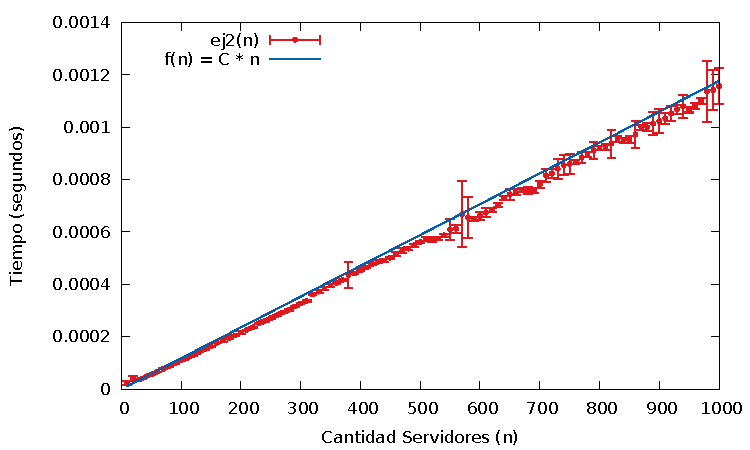
\includegraphics{imgs/ej2_1000_10_100.pdf}
\caption{Test Performance: Tiempo(s) vs Cantidad de Servidores}
\end{figure}

Notar que los tiempos de ejecución se incrementan linealmente en función de la cantidad de servidores.
 
\subsection{Preguntas Adicionales}

\textbf{1 - }  \emph{Mostrar con un contraejemplo que es posible resolver las dos partes por separado de manera óptima pero que aun así haya una solución en la que la replicación termine en menos tiempo. Comentar posibles soluciones al problema.}\\

Podemos ver el siguiente ejemplo, supongamos que tenemos el grafo: 

\begin{figure}[H]
\centering
\def\svgwidth{140 pt}
\input{imgs/ejemploEj2_b.pdf_tex}
\end{figure}

Se puede ver que tenemos dos árboles generadores mínimos. 

\begin{figure}[H]
\centering
\def\svgwidth{200 pt}
\input{imgs/ejemploEj2_b2.pdf_tex}
\end{figure}

Nuestro procedimiento devuelve el árbol de la izquierda. No obstante, el de la derecha tiene un tiempo de broadcast mejor más chico.  

\textbf{2 - }  \emph{¿Cómo se debe modificar la solución si en lugar de transmitir por broadcast se lo hace por multicast, es decir, se debe mandar un paquete a cada destino, sin hacer copias?}\\

Habría que modificar el ejercicio 2-B únicamente. En la versión del problema que funciona por broadcast nos importa buscar el nodo que garantice que el tiempo de broadcast total sea el menor posible. Si lo hacemos por multicast entonces tenemos que enviar el dato a todos los nodos, una vez a cada uno. Esto significa recorrer todos los caminos del árbol posibles para llegar hasta cada nodo. Deberíamos modificar la solución del ejercicio para que esta recorra todos los caminos hasta todos los nodos posibles, lo cual podemos hacer con una versión modificada de DFS, que guarde todos los caminos que vamos recorriendo para llegar a cada nodo.


\newpage
\section{Ejercicio 3}
\subsection{Interpretación del enunciado}
\par{En cierta provincia se ubican varias fábricas de ladrillos pertenecientes
  una misma empresa. La empresa se encarga de distribuír  lo s ld rillos de l
as fábricas a sus clientes. Para ello, utiliza las rtas provinciales que conec                                                                                                                                                                                                                                                                                         
distintos puntos de la provincia en los que puede haber una fábrica o un
cliente. Sin embargo, las rutas no están preparadas para soportar el peso de
los camiones que transportan los ladrillos, así que estas deben ser
fortalecidas. El costo de fortalecer cada ruta es proporcional a la longitud de
la misma. La empresa quiere fortalecer determinadas rutas para poder distribuír
los ladrillos a sus clientes sin problemas, intentando reducir lo más posible
el costo de dicha remodelación. El objetivo del ejercicio es desarrollar un
algoritmo que determine el conjunto de rutas que deben ser fortalecidas para
poder continuar la distribución (debe haber una ruta fortalecida entre cada
cliente y al menos una fábrica), cuyo costo de fortalecimiento sea mínimo.}
\subsection{Resolución}
\par{Se modelará la situación a través de un grafo en el que cada nodo
representará un cliente o una fábrica y cada arista entre un par $v1$, $v2$
de nodos representará una ruta entre los clientes o fábricas correspondientes a
$v1$ y $v2$. Para modelar el costo de fortalecer cada ruta, se le asignará a
cada arista el peso equivalente a la longitud de su correspondiente ruta. Si
bien el grafo podría no ser conexo, Se asume que existe un camino simple entre
cada cliente y al menos una fábrica, ya que se parte de que se puede satisfacer
la demanda de todos los clientes. Se busca obtener un conjunto de rutas tal que
exista un camino entre cada cliente y al menos una fábrica, es decir que
debemos encontrar un subgrafo en el grafo modelado. Como se busca reducir el
costo total sería conveniente que dicho subgrafo esté compuesto por árboles.
Este subgrafo constaría de una componente conexa por cada fábrica, sin dejar
clientes afuera. Cada componente conexa tendría que ser un árbol generador
del subgrafo inducido por los nodos de dicha componente. De esta forma se está
asegurando mantener la mínima cantidad de rutas necesarias. De todos los
posibles subgrafos bosque, debemos tomar el de menor peso para reducir el costo
total de fortalecer las rutas. En definitiva hay que encontrar un bosque
generador (conjunto de árboles generadores) de peso mínimo en el grafo modelado,
con la restricción de que haya exactamente una fábrica en cada árbol y ningún
cliente quede afuera.

A continuación, se presenta el pseudocódigo del algoritmo:\\

\begin{algorithm}[H]
	\caption{Algoritmo de Ejercicio 3}
	\KwData{Grafo G=(V,E) con nodos clientes y nodos fábrica, tal que para todo cliente, hay una fábrica alcanzable desde el.}
	
	$G.aristas \longleftarrow$ ordenar$\_$por$\_$peso$\_$asc($G.aristas$)\\
	\textbf{vector<arista>} $res \longleftarrow \emptyset$\\
	\ForEach{$e \in G.aristas$}{
		\If{!forma$\_$ciclo($e$, $res$) $\land$ no une dos componentes con una fábrica en cada una}{
		$res \longleftarrow res \cup e$\\
		}
	}
	\textbf{return} $res$\\
	
\end{algorithm}

}

\subsection{Demostración de Correctitud}


\textbf{La solución es válida:\\}
    Demostración:
    Todo cliente puede ser provisto por al menos una fábrica ya que hay una
    fábrica por componente conexa.
    Veremos que el algoritmo retorna un grafo $G $con cada cliente que pertenece a una componente
    conexa(en la que hay una fábrica):\\
    Supongamos que hay un cliente $c$ que no está en ninguna componente conexa. Esto es equivalente a afirmar
    que $c \notin V(G)$. Como cada cliente en el grafo de entrada del algoritmo, tiene un camino a alguna fábrica
    $\Longrightarrow$ existe un camino entre cualquier cliente y alguna fábrica.}

\textbf{Demostrar que es óptimo}

    \par{
%   \textbf{Demostrar que existe una solución óptima con una fábrica por componente conexa:}
    
    Notar que la solución debe cumplir que en cada componente conexa hay al menos una fábrica. Veremos que si un grafo $G$ contiene
    más de una fábrica en una componente conexa, existe un subgrafo (con el mismo conjunto de vertices y menos aristas)
    de $G'$ con una sola fábrica por componente conexa con menor peso que el de $G$.
    
    \textbf{Propiedad:} Sea una $G$ el grafo de una solución con más
    de una fábrica en alguna componente conexa, veremos que si hay una sola fábrica en esa componente, el costo de la nueva solución
    quitandole una arista \footnote{Esta arista que quitamos pertence a un camino entre dos fábricas}tiene igual o menor peso.\\
    
    Demostración:
    Sea $P$ un camino entre dos fábricas y sea $G'$ el grafo resultante de quitarle una arista $e$ (que une a los nodos $u,v$)
    perteneciente a un camino entre dos fábricas:$ P = C_1 \leftrightarrow (u,v) \leftrightarrow C_2$.
    Veamos que $G'$ sigue siendo solución posible.
    
    Sea un nodo cliente que no está en la componente conexa a la que pertenece $e$. Luego, ese cliente tiene a una fábrica alcanzable,
    ya que no quitamos ninguna arista de su componente conexa y como $G$ era solución, había una fábrica en esa componente.
    Sea un nodo cliente $c$ que estaba en la componente conexa a la que pertenece $e$.
    En ese caso como $G$ era un grafo solución, existia en $G$ un camino entre un c y una fábrica. Luego en ese camino, pasaba por
    $u$, o por $v$ (los nodos incidentes a la arista removida).Sin perdida de generalidad, supongamos que inicidía en v.
    
    Como $e$ era una arista que pertenecía a un camino entre dos fábricas se puede crear un camino
    que llegue desde $c$ a una fábrica: $ c \leftrightarrow v \leftrightarrow C_2$. Luego $G'$ tambien es solución.
    Además como quitamos una arista, que tiene peso positivo (todas lo tienen), el costo
    de la solución es menor o igual a la solución anterior.
    
    Esta quita de aristas se puede repetir hasta tener un grafo con una fábrica por componente conexa. Este grafo
    sera solución optima pues no se le pueden quitar aristas: si se remueve una arista de una componente conexa (que es un arbol) 
    la cual contiene una sola fábrica , se va a desconectar la componente generando asi la imposibilidad
    para algun cliente de alcanzar a la fábrica que estaba en la componente conexa (antes de quitar la arista).\\}

% 	\par{\textbf{Demostrar que usa la cantidad mínima de aristas:}
% 	Sea T una solución con una fábrica por componente conexa(cc) y c aristas (la cantidad de cliente).
% 	Como cada cc es una AGM, al quitar una arista de una cc, pasan a haber 2 ccs, y como sólo había una fábrica por cc,
% 	los clientes de alguna de las 2 ccs formadas no podrá ser provisto.
% 	$\Rightarrow$ La cantidad de aristas de la solución es mínima.}

  \par{
  \textbf{El peso de la solución es mínimo:\\} 
  Demostración:\\
  Sea $T$ la solución devuelta por nuestro algoritmo y sea $e$ una arista del grafo original tal que $e \notin T$.
  Agrego la arista $e = (u,v)$ a $T$ generando así al grafo $T'$:

  \textbf{Caso 1, $u$ y $v$ pertenecen a la misma cc en T: } 
  Cada cc del grafo devuelto por nuestro algoritmoes un AGM y, por ser árbol,
  $T+e$ contiene un ciclo incluído en la cc de $u$ y $v$. Sea $C$ tal ciclo, tomo $f$
  arista en $C$. Defino $T' = T+e-f$ con peso $p(T') = p(T) + p(e) - p(f)$.
  Como nuestro algoritmo siempre selecciona las aristas de peso minimo que no forman ciclo
  $$p(f) \leq p(e)$$ , luego
  $$0 \leq p(e) - p(f) \Rightarrow p(T') \geq P(T)$$. Es preciso aclarar que $T+e-f$ es conexo, por lo tanto todos los clientes
  tienen a una fábrica alcanzable.

  \textbf{Caso 2, $u$ y $v$ pertenecen a distintas cc en T: }
  Las ccs de $u$ y $v$ ahora son una misma cc con dos fábricas. Esta cc es un árbol porque es conexa (obvio) y la cantidad de
  aristas es la suma de la cantidad de aristas es $m = m1+m2+1 = n1-1 + n2-1 +1 = n1+n2-1 = n-1$.
  Luego puedo quitar una arista que pertenece al camino entre las dos fábricas \footnote{Es preciso aclarar que puedo suponer esto de la arista
  que quitamos ya que nuestro algoritmo no devuelve grafos con componentes conexas con más de una fábrica.}
  que actualmente están conectadas con el  camino
  $ P = C_1 \leftrightarrow (u,v) \leftrightarrow C_2$. Luego cualquier cliente del grafo resultante de remover la arista $e$
  tiene un camino hasta alguna fábrica:
  
  Sea un nodo cliente que no está en la componente conexa a la que pertenece $e$. Luego, ese cliente tiene a una fábrica alcanzable,
  ya que no quitamos ninguna arista de su componente conexa y como $T$ era solución, había una fábrica en esa componente.
  
  Sea un nodo cliente $c$ que estaba en la componente conexa a la que pertenece $e$.
  En ese caso como $T$ era un grafo solución, existia en $T$ un camino entre un c y una fábrica. Luego en ese camino, pasaba por
  $u$, o por $v$ (los nodos incidentes a la arista removida).Sin perdida de generalidad, supongamos que inicidía en v.
    
  Como $e$ era una arista que pertenecía a un camino entre dos fábricas se puede crear un camino
  que llegue desde $c$ a una fábrica: $ c \leftrightarrow v \leftrightarrow C_2$. Luego $T'$ tambien es solución.
    
  Como nuestro algoritmo siempre selecciona las aristas de peso minimo que no forman ciclo
  $$p(f) \leq p(e)$$ , luego
  $$0 \leq p(e) - p(f) \Rightarrow p(T') \geq P(T)$$.
    
% 		Como la cantidad de aristas
% 		de la solución actual es una más que la mínima puedo sacar una arista de la nueva cc para obtener una solución mejor que
% 		T+e, siempre y cuando mantenga que las dos ccs que se formen al quitar una arista de la nueva cc, tengan una fábrica.
% 		Sea f una arista distinta de e tal que al quitarla de la nueva cc, se formen dos ccs con una fábrica cada una (Si no hubiese
% 		una f distinta de e, tendría que sacar e y volvería a quedar la misma solución, por lo tanto sería solución única).
% 		el peso de f no puede ser mayor al peso de e porque si lo fuera, en lugar de escoger f, el algoritmo habría escogido e.\\
}


    $\Rightarrow$ Cualquier solución del tipo $T+e-f$ tiene peso mayor o igual al peso de $T \Rightarrow$ Nuestra solución es óptima. \box

}

\end{enumerate}

%\subsection{Complejidad}
%La complejidad del algoritmo es $O(m+n)$, ya que se fija en todas las aristas

\subsection{Cota de Complejidad}

\subsection{Implementación}

\begin{lstlisting}
grafo kruskal(){
  disjointSet ds(this->cantNodos);
  vector<arista> res;
  /*Ordeno la lista de aristas para Kruskal */ // ----> O(n logn)
  sort(this->aristas.begin(), this->aristas.end()); 
  
  int i = 0;	//indice de arista que itero
  int j = 0;	//Cantidad de aristas que agregue
  int cantClientes = cantNodos - this->cantFabricas;
  
  while (j < cantClientes){
    int root1 = ds.root(this->aristas[i].nodo1)->valor;
    int root2 = ds.root(this->aristas[i].nodo2)-> valor;
    if((root1 != root2) 	//estan en distintas componente conexas y...
    // no pasa que ambos tengan una fabrica
    && !((root1 < this->cantFabricas) && (root2 < this->cantFabricas)) ){ 
      if (root1 < this->cantFabricas) {  //Si el primero es una fabrica...
	      ds.simple_join(root2, root1);      
      } else {   //Si el segundo es fabrica o si ninguno lo es.
	      ds.simple_join(root1, root2);	     
      }
      j++;
      res.push_back(this->aristas[i]);
    }
    i++;
  }
  
  /* Armo el grafo para devolver */
  grafo g_res(this->cantNodos);
  for(int i = 0; i < res.size(); ++i)
	  g_res.asociar(res[i].nodo1+1, res[i].nodo2+1, res[i].peso);
  
  return g_res;
}
\end{lstlisting}
\newpage


\subsection{Testing de Correctitud}

Los tests expuestos a continuación fueron diseñados con el fin de verificar
diferentes casos particulares que pudimos identificar. Para cada test vamos
a exponer la entrada, la salida y, en caso de que sea necesario, una
justificaci\'on de la correctitud de la soluci\'on.\\

\noindent\textbf{Test$\#$1}\\
\textbf{Caracterización:} Una fábrica sin clientes.\\
\textbf{Input:}\\ \texttt{1 0 0}
\begin{center}
\begin{dot2tex}
graph graphname{
	rank=same;
	rankdir="LR";
	splines=line;
	1;
}
\end{dot2tex}
\end{center}
\textbf{Output:} \texttt{0 0}\\
\textbf{Status:} Ok, como no hay clientes, no hay rutas que fortalecer.\\

\noindent\textbf{Test$\#$2}\\
\textbf{Caracterización:} Varias fábricas sin clientes.\\
\textbf{Input:}\\ \texttt{6 0 8\\1 2 5\\1 3 7\\2 3 3\\2 4 6\\3 4 8\\
4 5 8\\4 6 4\\6 1 2}
\begin{center}
\begin{dot2tex}
graph graphname{
	rank=same;
	rankdir="LR";
	splines=line;
	1 -- 2 [label=5];
	1 -- 3 [label=7];
	3 -- 2 [label=3];
	4 -- 2 [label=6];
	4 -- 3 [label=8];
	5 -- 4 [label=8];
	4 -- 6 [label=4];
	1 -- 6 [label=2];
}
\end{dot2tex}
\end{center}
\textbf{Output:} \texttt{0 0}\\
\textbf{Status:} Ok, como no hay clientes, no hay rutas que fortalecer.\\



\noindent\textbf{Test$\#$3}\\
\textbf{Caracterización:} Varias fábricas y un cliente.\\
\textbf{Input:}\\ \texttt{4 1 8\\1 2 5\\1 3 7\\2 3 3\\2 4 6\\3 4 8\\
4 5 8\\4 1 4\\5 2 2}
\begin{center}
\begin{dot2tex}
graph graphname{
	rank=same;
	rankdir="LR";
	splines=line;
	1 -- 2 [label=5];
	1 -- 3 [label=7];
	3 -- 2 [label=3];
	4 -- 2 [label=6];
	4 -- 3 [label=8];
	5 -- 4 [label=8];
	4 -- 1 [label=4];
	2 -- 5 [label=2];
}
\end{dot2tex}
\end{center}
\textbf{Output:} \texttt{ 2 1 5 2}\\
\textbf{Status:} Ok, como hay un solo cliente (el nodo 5), elige la ruta de costo minimo que conecta
 a ese cliente con una de las fábricas(el nodo 2) adyacentes.\\

\noindent\textbf{Test$\#$4}\\
\textbf{Caracterización:} Varios clientes y una fábrica.\\
\textbf{Input:}\\ \texttt{1 4 8\\1 2 5\\1 3 7\\2 3 3\\2 4 6\\3 4 8\\
4 5 8\\4 1 4\\5 2 2}
\begin{center}
\begin{dot2tex}
graph graphname{
	rank=same;
	rankdir="LR";
	splines=line;
	1 -- 2 [label=5];
	1 -- 3 [label=7];
	3 -- 2 [label=3];
	4 -- 2 [label=6];
	4 -- 3 [label=8];
	5 -- 4 [label=8];
	4 -- 1 [label=4];
	2 -- 5 [label=2];
}
\end{dot2tex}
\end{center}
\textbf{Output:} \texttt{14 4 5 2 2 3 4 1 1 2 }\\
\textbf{Status:} Ok, como hay una sola fábrica debe conectar a todo el grafo(fábrica y clientes) con el menor costo posible.
Es decir debe hacer el AGM del grafo. Notar que lo hace ya que devuelve lo que haria Kruskal, siempre eligiendo los nodos de menor peso
que no generan circuitos.\\

\newpage
\subsection{Testing de Performance}

Para realizar el test, generamos grafos aleatorios, con pesos aleatorios (entre 0 y 100). Decimos que los grafos son aleatorios, porque nuestro algoritmo va agrandando alguna componente conexa uniendo vertices
correspondientes a los clientes con componenetes conexas que contienen una fabrica. Cabe destacar que esas componenetes conexas pueden ser simplemente una fábrica.

Realizamos un gráfico comparando la sucesión de tiempos obtenida con una función cuadrática.
La función $f = C * n^2$, donde C es una constante. Se midió el tiempo con n desde 1 hasta 1000 con saltos de a 10 (con 10 mediciones por cada n).\\

\begin{figure}[H]
\centering

\includegraphics{imgs/logo_dc.jpg}
\caption{Test Performance: Tiempo(s) vs Cantidad de Clientes y Fábricas.}
\end{figure}


\newpage
\section{Conclusiones}

 
\end{enumerate}
 En primera instancia, la realización del primer ejercicio nos permitió familiarizarnos con el proceso de desarrollo de una solución utilizando la técnica de programación dinámica:
\begin{enumerate}
 \item Caracterizamos la estructura de una solución óptima.
 \item Definimos el valor de la solución óptima recursivamente.
 \item Computamos el valor de la solución óptima, con una estrategia bottom-up .
 \item Construimos la solución óptima con la información computada.
\end{enumerate}
 
Por otro lado, los ejercicios 2 y 3 nos permitieron acercarnos de manera introductoria al modelado de problemas utilizando conceptos de teoría de grafos. El proceso de desarrollo nos impuso la necesidad de contemplar diferentes modelos para cada problema y analizar cuales de estos representaban el problema de manera correcta. 

Luego, utilizando la bibliografía sugerída por la materia y las clases teóricas de la misma, pudimos contemplar diferentes algoritmos y terminamos decidiendo un curso de implementación que en principio pareciera satisfactorio. Durante el proceso de desarrollo los algoritmos implementados fueron cambiados en varios puntos para hacerlos más compatibles con el problema en si. 

A su vez, tuvimos que investigar tanto diferentes opciones de estructuras de datos a la hora de implementar grafos, como diferentes estructuras auxiliares para los algoritmos. En algunos casos incluso realizamos una serie de tweaks a las estructuras empleadas para adaptarlas a nuestros algoritmos y que estos cumplieran bien las cotas de complejidad impuestas por el enunciado.

Por el costado formal, las justificaciones de nuestras soluciones nos sirvieron para complementar las ejercitaciones de la práctica de la materia; contemplando diferentes técnicas de demostración para verificar la correctitud de nuestras implementaciones.

En resumen, creemos que el desarrollo de este trabajo práctico cumplió un rol fundamental dentro del programa de la materia y fue un buen complemento para las clases teóricas y prácticas de la misma.

\newpage
\section{Informe de modificaciones para la reentrega}

\subsection{Pautas de Implementación}
\textbf{Clase GrafoEx}
\par{A pesar de no haberlo mencionado en la primera entrega, se desarrollaron
en realidad dos clases basadas en grafos. La primera, definida en $grafo.h$
es un grafo estándar utilizado para el ejercicio 2. La segunda, definida en
$grafoEx.h$ representa un grafo con nodos diferenciables, utilizado para el
ejercico 3. La mayor parte de las funciones son idénticas en ambas clases,
aunque la función para generar una AGM a partir del algoritmo de $Kruskal$,
en el caso de grafoEx, en lugar de generar un árbol, genera un bosque con
un nodo diferenciable en cada componente conexa. Para representar la provincia
del ejercicio 3, representamos las fábricas con los nodos diferenciables y
los clientes con los nodos no diferenciables. Además, $grafoEx$ tiene una
variante del algoritmo de $Kruskal$, llamada $Kruskal\_no\_res$ la cual
hace lo mismo que la función de $Kruskal$ pero no devuelve el resultado.}

\textbf{Disjoint Set}
\par{Otra clase desarrollada que tampoco fue mencionada en la primera entrega
es la implementada en $disjointSet.h$. Esta clase se basa en...}

\textbf{Tests corregidos}
\par{En la primera entrega los tiempos medidos con $test.cpp$ fueron muy poco
precisos debido a que, al medir el tiempo de ejecución de cada $resolver\_x$
estábamos incluyendo el código correspondiente a inicializar las estructuras de
los resultados y, en algunos casos copiarlas. Para resolverlo, modificamos
el archivo $tests.cpp$ para que cada función $testear\_ejx$, en lugar de hacer
una llamada a $resolver\_ejx$, ejecute las mismas funciones que esta última
pero sin guardarse ni devolver los resultados obtenidos. En el ejercicio 3
se utilizó la función $Kruskal\_no\_res$ en lugar de $Kruskal$ con este
objetivo. Como se editó el archivo $tests.cpp$, se rehicieron todos los
gráficos.}
\par{Para mayor claridad, la función $generar\_instancia\_ej2$ fue reemplazada
por $generar\_instancia\_ej2b$, ya que en realidad, esta función generaba una
instancia de entrada para la parte $b$ del ejercicio, es decir un árbol.
Asimismo, la función $generar\_aristas\_aleatorias$ de $grafo.h$ genera en
realidad un árbol para ser utilizado como entrada del ejercicio. En el caso del
$grafoEx$, $generar\_aristas\_aleatorias$ genera un grafo no necesariamente
conexo, aunque sí asegurando que todo cliente está en una componente conexa
en la que hay al menos una fábrica. Luego, para cada arista posible, elige
al azar (con probabilidad 0.5) si agregarla o no al grafo; Por lo que la
cantidad de aristas de entrada para el ejercico 3 es, en promedio $n.(n-1)$ / 4.}

\textbf{Código}
\par{Además de algunos cambios menores en el código, se quitaron todas las
utilizaciones de $new$ y ahora todos los parámetros se pasan por referencia,
en lugar de hacerse por copia. También cambiamos el $Makefile$ quitándo el
flag -O2 para obtener mediciones más estables.}
\subsection{Ejercicio 1}
\textbf{Testing de performance}
\par{Se rehizo el gráfico en función de los cambios realizados en $tests.cpp$.
También ampliamos el análisis del mismo.}
\subsection{Ejercicio 2 - A}
\textbf{Resolución}
\par{Se agregó a la explicación de la resolución del ejercicio una idea del
funcionamiento del algoritmo de $Kruskal$}

\textbf{Demostración de correctitud}
\par{Se agregó la sección faltante en la primera entrega en la que demostramos
la correctitud del ejercico a partir de la demostración de correctitud del
algoritmo de $Kruskal$}

\textbf{Cota de Complejidad}
\par{Se agregó la sección faltante en la primera entrega en la que demostramos
la cota de complejidad del ejercico a partir de la complejidad del
algoritmo de $Kruskal$}

\textbf{Implementación}
\par{Se reescribió esta sección profundizando en la implementación del
algoritmo de $Kruskal$ y de la clase $disjointSet$.}

\subsection{Ejercicio 2 - B}
\textbf{Resolución}
\par{Se agregó una idea del funcionamiento de los algoritmos de recorrido de
grafos, $BFS$ y $DFS$ utilizados para la resolución del problema.}

\textbf{Implementación}
\par{Se reescribió esta sección profundizando en la implementación de los
algoritmos de $BFS$ y $DFS$ utilizados.}

\textbf{Testing de performance}
\par{Se rehizo el gráfico en función de los cambios realizados en $tests.cpp$.
También ampliamos el análisis del mismo.}
\subsection{Ejercicio 3}
\textbf{Cota de Complejidad}
\par{Se agregó la sección faltante en la primera entrega en la que demostramos
la cota de complejidad del ejercico a partir de la complejidad del
algoritmo de $Kruskal$}

\textbf{Testing de correctitud}
\par{Se rehicieron los gráficos que muestran las instancias pero los tests
son los mismos.}
\end{document}

\textbf{Testing de performance}
\par{Se rehizo el gráfico en función de los cambios realizados en $tests.cpp$.
También ampliamos el análisis del mismo.}
\end{document}
